
%(BEGIN_QUESTION)
% Copyright 2006, Tony R. Kuphaldt, released under the Creative Commons Attribution License (v 1.0)
% This means you may do almost anything with this work of mine, so long as you give me proper credit

Forklar hvordan den vertikale høyden av en væske kan skape trykk, slik som i dette eksempelet:

$$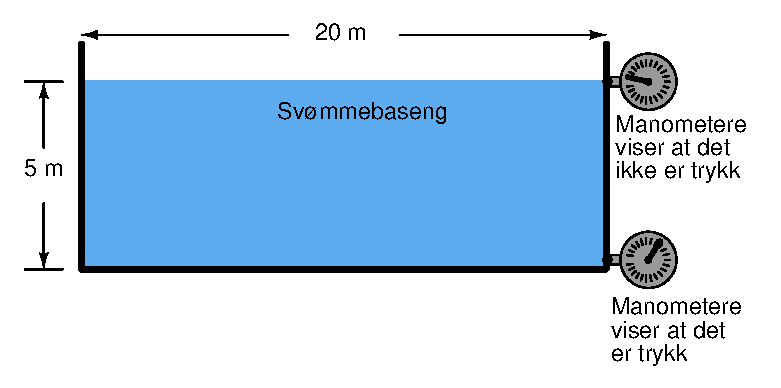
\includegraphics[width=14cm]{i00749x01.eps}$$

Jo dypere du kommer i vannet, desto høyere blir trykket.

\vskip 10pt

Husk at trykk er definert som kraft per areal:

$$P = {F \over A}$$

Regn ut den totale vekten av vannet i dette svømmebassenget. Bassenget er rundt og har en diameter på 20 m. Regn også ut trykket i bunnen av bassenget.

\vskip 10pt

Vekten av vannet = \underbar{\hskip 50pt} kg

\vskip 10pt

Trykket i bunnen av bassenget = \underbar{\hskip 50pt} bar

\vskip 10pt

\underbar{file i00749}
%(END_QUESTION)





%(BEGIN_ANSWER)

Vekt av vann = \underbar{53\,377} kg

\vskip 10pt

Areal av sirkulær bassengbunn = 45\,239 in$^{2}$

\vskip 10pt

Trykk i bunnen av bassenget = $P$ = 2.601 lb/in$^{2}$ (PSI) = 72 inches vannsøyle (" W.C.) $\approx$ 0.179 bar

\vskip 10pt


%(END_ANSWER)





%(BEGIN_NOTES)


%INDEX% Fysikk, statiske væsker: hydrostatisk trykk

%(END_NOTES)


